\documentclass{standalone}
\usepackage{textcomp}
\usepackage{pgfplots}
\begin{document}
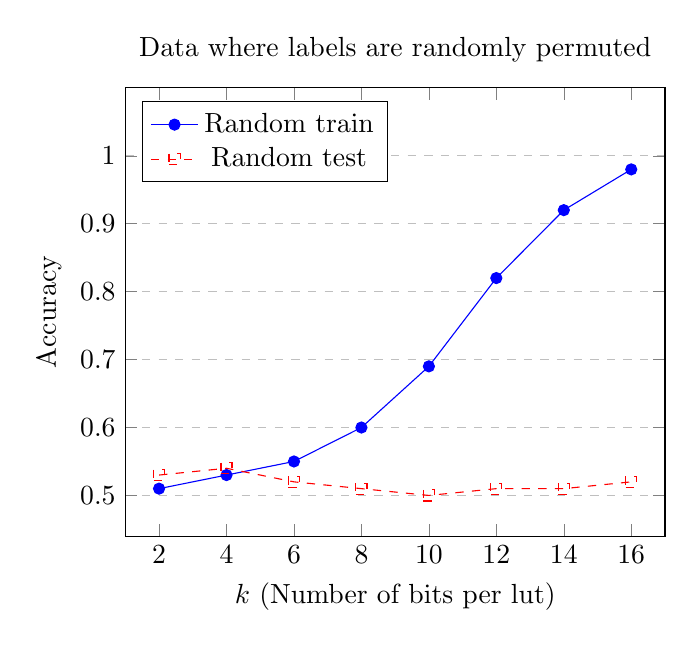
\begin{tikzpicture}
\begin{axis}[
    title={Data where labels are randomly permuted},
    xlabel={$k$ (Number of bits per lut)},
    ylabel={Accuracy},
    xmin=1, xmax=17,
    ymin=0.44, ymax=1.1,
    xtick={2,4,6,8,10,12,14,16},
    ytick={0.5,0.6,0.7,0.8,0.9,1.00},
    legend pos=north west,
    ymajorgrids=true,
    grid style=dashed,
]

\addplot[
    color=blue,
    mark=*,
    ]
    coordinates {
        (2,0.51)(4,0.53)(6,0.55)(8,0.60)(10,0.69)(12,0.82)(14,0.92)(16,0.98)
    };
    \addlegendentry{Random train}

\addplot[
    color=red,
    mark=square,
    dashed,
    ]
    coordinates {
        (2,0.53)(4,0.54)(6,0.52)(8,0.51)(10,0.50)(12,0.51)(14,0.51)(16,0.52)
    };
    \addlegendentry{Random test}
    
\end{axis}
\end{tikzpicture}
\end{document}
